\documentclass[xcolor=dvipsnames]{beamer}
%\usecolortheme[named=RoyalBlue]{structure}
%\usecolortheme[named=CornflowerBlue]{structure}
\usecolortheme[named=Red]{structure}
%\usetheme{Antibes}
%\usetheme{Singapore}
\usetheme{Berlin}

\usepackage[utf8]{inputenc}
\usepackage{times}
\usepackage[T1]{fontenc}

\usepackage{graphicx}

\setbeamertemplate{blocks}[shadow=true] 
\setbeamertemplate{navigation symbols}{} 

\title[RDBMS Over FreeBSD]{Advocacy for the OpenSource Relational Data Base Management System Over FreeBSD}
\author{Jorge A. Medina - Santiago/Chile}

\institute{Computer Science Research Crew\\ http://www.bsdchile.cl \scriptsize{\textcircled{\tiny{R}}}}
%\mode<presentation>

\date{Feb. 20 , 2009}

\AtBeginSection[]
{
	\begin{frame}<beamer>
		\frametitle{Index}
		\tableofcontents[currentsection]
	\end{frame}
}

\begin{document}
\fontsize{7}{9}
	\begin{frame}
		\titlepage
	\end{frame}

\section{FreeBSD Introduction}
	\begin{frame}{Way FreeBSD?}
		\begin{enumerate}
			\item The BSD license it's realy "Free" this it's important.
			\item The OS is released under BSD license \\other important products like PostgreSQL too.
			\item Installing easy and fast.
			\item Upgrading easy bandwidth-depended but realy fast\\(freebsd-update,csup,portupgrade).
			\item Software necesary ports tree (portsanp fetch,extract,update).
			\item Easy Kernel build (make buildkernel, make installkernel).
			\item Easy User Land build (make buildworld, make installworld).
			\item Basic Virtualization or chrooted environment \\more secure with FreeBSD Jails.
			\item Basically the core it's realy realy more powerfull than others OS.
					\\ Branch-7 Re-designed the FreeBSD kernel 
					\\ as a multi-threaded system for "next generation" SMP support
			\item And many many others.
		\end{enumerate}
	\end{frame}
	
\section{FreeBSD Test's}
	\begin{frame}{How it's possible\footnote{\tiny{Source: Kris Kennaway FreeBSD Project committer since 1999.}}?}
	\begin{itemize}
		\item FreeBSD 7.0 was released, and the first major release in 2 years.
		\item FreeBSD 7.1 brings major changes to the BSD and open source operating system landscape.
		\item FreeBSD 8.0 comming soon, it's the current available for testing
	\end{itemize}
	\begin{quote}{The begin}
	{
		\\"Last week, approximately 20 BSD developers got together and discussed
		how to move FreeBSD's SMP support to the next level. 
		Our effort will be largely based on the work that has been done in BSD/OS, which
		should make things go much more smoothly than they otherwise might, 
		but we still expect -current to be destabilized for an extended period of time."\\
		(Jason Evans, email to freebsd-current list, 19 June 2000.)
	}
	\end{quote}
	\end{frame}
	\begin{frame}{The Result}
	\begin{itemize}
		\item \textbf{Goal:} Re-design the FreeBSD kernel as a multi-threaded system,
			for "next generation" SMP support (June 2000).
		\item Multiple CPUs must be able to execute kernel code in parallel
		\item Balance the performance needs of Uni-Processor (UP) and SMP systems (not always different needs)
		\item A major challenge...
		\item ...now complete
	\end{itemize}
	\end{frame}
	
	\begin{frame}{SQL DataBase Performance}
	\begin{itemize}
		\item "Online transaction processing" benchmark; /usr/ports/benchmarks/sysbench
		\item Transaction-based queries
		\item Read-only: no disk access to avoid benchmarking disk performance
		\item Clients and servers on the same system
		\item PostgreSQL 8.2.4 (process-based + System 5 Inter-Process Communication (IPC)
		\item MySQL 5.0.45 (thread-based)
		\item Test hardware:
		\begin{itemize}
		\tiny 
		{
			\item 2-core Opteron (amd64 mode) 2.2GHz CPUs, 4 GB RAM
  			\item 4-core Xeon E5320 (i386 mode) 1.8GHz CPUs, 3.5GB RAM
  		}
  		\end{itemize}
	\end{itemize}
	\end{frame}
	
	\begin{frame}{Performance Of PostgreSQL}
	\begin{itemize}
	\item The ULE scheduler has significantly better performance \\than old 4BSD (historical BSD scheduler)\\
    \begin{itemize}
    \tiny
    {
     	\item Better interactivity for desktop users also
     	\item 4BSD will remain the default in 7.0, changing in 7.1
     	\item You can easily switch to ULE by recompiling your kernel
   	}
    \end{itemize}
    \item PostgreSQL with ULE has linear scaling to 8 CPUs and minimal degradation at higher loads; 
    	\\ close to ideal performance from the hardware.
	\item No significant performance problems in the FreeBSD 7 kernel on this workload
	\end{itemize}
	\end{frame}
	
	\begin{frame}{\scriptsize{Scaling with varying number of CPUs}}
	\begin{figure}
	\centering 
		\includegraphics[scale=0.32]{graf01.eps} 
	\end{figure}	
	\end{frame}
	
	\begin{frame}{\scriptsize{\textbf{Note:} Scaling with varying number of CPUs}}
	\begin{itemize}
		\item Performance from 1  2  4  8 CPUs scales linearly
		\item Consistently stable performance at high loads
		\item No significant overhead from SMP kernel on UP system
	\end{itemize}
	\end{frame}
		
	\begin{frame}{\scriptsize{FreeBSD vs other operating systems: PostgreSQL}}
	\begin{figure}
	\centering 
		\includegraphics[scale=0.32]{graf02.eps} 
	\end{figure}
	\end{frame}

	\begin{frame}{\scriptsize{FreeBSD vs other operating systems: MySQL}}
	\begin{figure}
	\centering 
		\includegraphics[scale=0.32]{graf03.eps} 
	\end{figure}
	\end{frame}
		
	\begin{frame}{\scriptsize{MySQL performance}}
	\begin{itemize}
		\item Again, linear scaling up to 8 client threads (= \# CPUs)
		\item The degradation above 8 threads is due to scaling problems within MySQL (not a FreeBSD kernel issue)
		\item Heavy contention on pthread mutexes within the application
		\item Recent change to libpthread to reduce the performance loss from heavily contended pthread mutexes
		\begin{itemize}
		\tiny
		{
		    \item Non-portable "adaptive" mutex type defined by glibc, used by MySQL
		}
		\end{itemize}
		\item Ultimately a MySQL architectural problem
		\item On this benchmark PostgreSQL is 35\% - 45\% faster than MySQL at all loads
	\end{itemize}
	\end{frame}

	
\section{OS Performance Settings}
	\begin{frame}{TCP Tuning}
	\scriptsize
	{
	\begin{tabbing}
		---- \= ------ \= ------------------ \= ------------------------ \=  ... \kill
		Add these to \textbf{/etc/sysctl.conf} \\ \\
		\> kern.ipc.maxsockbuf=16777216 \\
		\> net.inet.tcp.rfc1323=1 \\
		\\ FreeBSD 7.x added TCP send and receive buffer autotuning.
		\\ There are some additional settings to modify.
		\\ (The default for these is 256 KB, which is too small):\\ \\
		\> net.inet.tcp.sendbuf\_max=16777216 \\
		\> net.inet.tcp.recvbuf\_max=16777216 \\
		\\ Here are some other new settings in 7.x to know about. Defaults for these should be fine.\\ \\
		\> net.inet.tcp.sendbuf\_auto=1    \>\>\> \# Send buffer autotuning enabled by default\\
		\> net.inet.tcp.sendbuf\_inc=8192  \>\>\> \# step size\\
		\> net.inet.tcp.recvbuf\_auto=1    \>\>\> \# enabled\\
		\> net.inet.tcp.recvbuf\_inc=16384 \>\>\> \# step size\\
	\end{tabbing}
	}
	\end{frame}

	\begin{frame}{TCP Tuning}
	\scriptsize
	{
	\begin{tabbing}
		---- \= ------ \= ------------------ \= ------------------------ \=  ... \kill
		FreeBSD's TCP has something called inflight limiting turned on by default. 
		\\ This is good for modem connections, but can be detrimental to TCP throughput in some 
		\\ high-speed situations. If you want "normal" TCP Reno-like behavior, set this:\\ \\
		\> net.inet.tcp.inflight.enable=0 \\
		\\ By default, FreeBSD caches connection details such as the slow start threshold and 
		\\ the congestion windows size from the previous connection to the same host for 1 hour. 
		\\ While this is a good idea for a web server, it makes it hard to do network throughput 
		\\ testing, as 1 large congestion event will throttle performance for the next hour. 
		\\ To reduce this effect, set this:\\ \\
		\> net.inet.tcp.hostcache.expire=1\\
		\\ This will still cache values for 5 minutes.
	\end{tabbing}
	}
	\end{frame}
		
	\begin{frame}{Important Options for DataBase Host}
	\scriptsize
	{
		\begin{tabbing}
		---- \= ------ \= ----- \= ... \kill
	    To have these settings persist over reboots, modify /etc/sysctl.conf. \\
		The remaining semaphore settings are read-only as far as sysctl is concerned, \\
		but can be changed before boot using the loader prompt: \\ \\
		
		\>(loader) set kern.ipc.semmni=256\\
		\>(loader) set kern.ipc.semmns=512\\
		\>(loader) set kern.ipc.semmnu=256\\ \\

		Similarly these can be saved between reboots in /boot/loader.conf. \\
		You might also want to configure your kernel to lock shared memory into RAM \\
		and prevent it from being paged out to swap. \\
		This can be accomplished using the sysctl setting \\ \\
		
		\> kern.ipc.shm\_use\_phys \\ \\
		
		\end{tabbing}
	}
	\end{frame}

	\begin{frame}{Important Options for DataBase Host}
	\scriptsize
	{ 
		\begin{tabbing}
		---- \= ------ \= ----- \= ... \kill		
		If running in FreeBSD jails by enabling sysctl's \\ \\
		
		\> security.jail.sysvipc\_allowed \\ \\
		
		Postmasters running in different jails should be run by different operating \\
		system users. This improves security because it prevents non-root users from \\
		interfering with shared memory or semaphores in a different jail, and it allows \\
		the PostgreSQL IPC cleanup code to function properly. (In FreeBSD 6.0 and later \\
		the IPC cleanup code doesn't properly detect processes in other jails, preventing \\
		the running of postmasters on the same port in different jails.)\\ \\		
		
		Others System Controls need tuning can be:\\ \\
		\>kern.ipc.shmall=32768 \\
		\>kern.ipc.shmmax=134217728 \\
		\>kern.ipc.semmap=256 \\\\
		\textbf{See:} Table 5.1
		\end{tabbing}
	}
	\end{frame}

\section{Mysql}
	\begin{frame}{MySQL}
	\scriptsize
	{
	\begin{tabbing}
		---- \= ------ \= ----- \= ... \kill
		MySQL dont have a complicated configuration with difficult decisions.\\
		But its important use InnoDB, instead MyIsam engine this can be set at CREATE command. \\
		It will set by default my.cf: \\ \\
		\> default\_table\_type = InnoDB \\ \\
		\textbf{Note:} Recent changes in libpthread, reduce the performance because\\
		can't portable "adaptive" mutex in glib pgsql IPC is 35\% more faster, only over FreeBSD.
		
	\end{tabbing}
	}
	\end{frame}

\section{PostgreSQL}

	\begin{frame}{PostgreSQL}
	\tiny
	{
	\begin{tabbing}
		---- \= ------------------ \= -------------------------------- \= ... \kill
		PostgreSQL ("pgsql" ahead) pgsql will require some manipulate parameters in some files \\
		after install like: \\ \\		
		(.cshrc) \\
		\>setenv  PGDATA  /usr/local/pgsql/data \\ \\
		\textbf{Now} pg\_ctl command work without -D flag\\ \\
		(postgresql.conf) \\
		\>max\_connections = 100 \\ 
		\>shared\_buffers = 32MB \>\>   \# min 128kB or max\_connections*16kB \\
        \>\>\>                          \# (change requires restart) \\
		\>temp\_buffers = 8MB \>\>		\# min 800kB \\
		\>\>\> \# Note:  Increasing max\_prepared\_transactions costs $\approx$600 bytes of shared memory \\
		\>\>\> \# per transaction slot, plus lock space (see max\_locks\_per\_transaction).\\
		\>work\_mem = 1MB                 \>\>        \# min 64kB\\
		\>maintenance\_work\_mem = 16MB      \>\>      \# min 1MB\\
		\>max\_stack\_depth = 2MB            \>\>     \# min 100kB\\
		\>max\_fsm\_pages = 204800 			\>\> \# min max\_fsm\_relations*16, 6 bytes each\\ \\
		(pg\_hba.conf)\\ \\

		\textbf{Note:} PostgreSQL don't used a posix thread to attend each of the incoming connections \\
		instead it use the complete instance of DataBase, this require specific tuning depending of 	\\ 
		system hardware (RAM) in this case. \\
	\end{tabbing}
	}
	\end{frame}
	
	\begin{frame}{PostgreSQL}
	\tiny
	{	 
	\begin{tabbing}
		---- \= ------ \= ----- \= ... \kill
		\textbf{Table 5.1:} System V IPC parameters
	\end{tabbing}
	\begin{center}
	\begin{tabular}{| l | l | l | }
		\hline
	    Name		& Description					& Reasonable values 						\\ \hline
	    
	    SHMMAX		& Maximum size of shared 		& at least several megabytes (see text)		\\
	    			& memory segment (bytes)  		&											\\ \hline
	    
	    SHMMIN		& Minimum size of shared 		& 1											\\
	    			& memory segment (bytes) 		&  											\\ \hline

		SHMALL 		& Total amount of shared memory	& if bytes, same as SHMMAX;					\\
					& available (bytes or pages) 	& if pages, ceil(SHMMAX/PAGE\_SIZE)			\\ \hline	
		
		SHMSEG 		& Maximum number of shared 		& only 1 segment is needed, 				\\
					& memory segments per process 	& but the default is much higher			\\ \hline

		SHMMNI		& Maximum number of shared 		& like SHMSEG plus room 					\\
					& memory segments system-wide 	& for other applications					\\ \hline

		SEMMNI 		& Maximum number of semaphore 	& at least ceil(max\_connections / 16)		\\ 
		       		& identifiers (i.e., sets) 		&											\\ \hline

		SEMMNS 		& Maximum number of      		& ceil(max\_connections / 16) \* 17 		\\
			   		& semaphores system-wide 		& plus room for other applications			\\ \hline
		
		SEMMSL 		& Maximum number of				& at least 17								\\
					& semaphores per set  			& 											\\ \hline

		SEMMAP 		& Number of entries 			& In some cases it might also be necessary 	\\
					& in semaphore map				& to increase in order to SMMNS (SMMNS/2)	\\ \hline

		SEMVMX 		& Maximum value of semaphore	& at least 1000 (The default is often 32767,\\
					& 								& don't change unless forced to)			\\ \hline

	\end{tabular}
	\end{center}
	}
	\end{frame}

	\begin{frame}{Resource Limits}
	\scriptsize
	{
	\begin{tabbing}
	---- \= ------------------ \= -------------------------------- \= ... \kill
	The file \textbf{/etc/login.conf} controls the various resource limits set during login.\\
	See the operating system documentation for details. The relevant parameters are maxproc, \\
	openfiles, and datasize. For example: \\ \\
	
	\>default:\textbackslash \\
	\>... \\
	\>\>	:datasize-cur=256M:\textbackslash \\
	\>\>	:maxproc-cur=256:\textbackslash \\ 
    \>\>	:openfiles-cur=256:\textbackslash \\
	\>... \\ \\

	(-cur is the soft limit. Append -max to set the hard limit.) \\
	Kernels can also have system-wide limits on some resources.  \\
	\end{tabbing}
	}
	\end{frame}


\section{The End}

	\begin{frame}{\scriptsize{Summary}} 
	\begin{itemize}
		\item FreeBSD 7.x and 8 brings FreeBSD back to the forefront of OS performance \\
		on modern hardware (it's good to be back).
		\item Provides advanced features not available in other open source operating systems.
		\item An attractive platform for high hardware.
		\item Better performance of RDBMS OpenSource like PostgreSQL and MySQL.
		\item Disponibility of many applications ports, from source(ports tree) and binary(packages).
		\item Good software management.
		\item and ZFS its coming :)
	\end{itemize}
	\end{frame}

	\begin{frame}{\scriptsize{More Information}}
	\begin{itemize}
		\item http://www.freebsd.org/
		\item http://people.freebsd.org/$\sim$kris/
		\item http://www.postgresql.org/
		\item http://www.bsdchile.cl/
	\end{itemize}
	\end{frame}
		
	\begin{frame}{\begin{center}THE END\end{center}} 
		\begin{center}
			Thanks for coming 
		\end{center}
	\end{frame}
\end{document}